\chapter{Resultados}

Para analisar o desempenho das implementações em Clojure e Haskell foi utilizada uma base de documento composta de 27 livros de domínio público em lingua inglesa que foram obtidos por meio do projeto Gutenberg\footnote{http://www.gutenberg.org/}, totalizando 18 \emph{megabytes} de arquivos texto. Foram utilizadas também cinco consultas com tamanhos distintos e ocorrências variadas na base de documentos. Os experimentos foram executados em uma máquina com processador Intel Core i7-3770 3.4GHz com 4 núcleos físicos e 8 \emph{gigabytes} de memória RAM rodando Linux. Para o ambiente Haskell foi utilizado o compilador GHC 7.6.2 junto com a \emph{flag} de compilação \verb|-O|. Já para o ambiente Clojure foi utilizado Clojure 1.5.1 com OpenJDK 7.u17.

\begin{figure}[h]
 \centering
 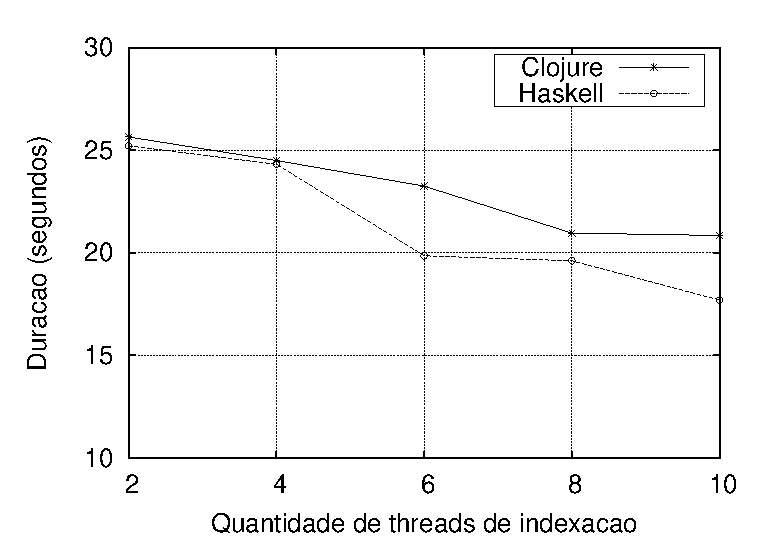
\includegraphics[scale=0.85]{imagens/clojure-haskell.eps}
 \caption{Gráfico do desempenho das versões paralelas em Clojure e Haskell}
 \label{fig:clj-hs-comp}
\end{figure}

A Figura \ref{fig:clj-hs-comp} mostra um gráfico onde o eixo horizontal representa a quantidade de \emph{threads} passada como argumento para o programa e o eixo vertical a duração em segundos da execução do programa. Cada ponto do gráfico representa a média do tempo de execução obtido a partir de 10 execuções consecutivas do programa calculado por meio do comando \verb|time| do Unix.

Como pode-se perceber o desempenho da implementação em Clojure foi consideravelmente pior que a implementação em Haskell. O comportamento das curvas é semelhante, mostrando que com o aumento da quantidade de \emph{threads} de indexação, o tempo total da execução do programa diminui. Isso mostra essa diferença entre o desempenho das duas implementações é um indicativo algum outro tipo de problema. Depois de alguma investigação, foi verificado, como mostra a Figura \ref{fig:clj-hs}, que a diferença de desempenho entre as versões sequenciais escritas em Clojure e Haskell também era bastante discrepante.

\begin{figure}[!h]
 \begin{minipage}{0.5\textwidth}
  \centering
  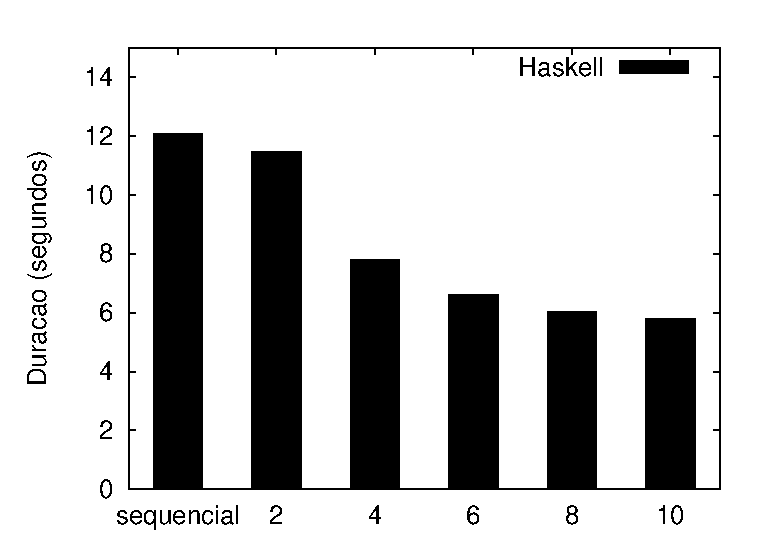
\includegraphics[scale=0.63]{imagens/haskell.eps}
 \end{minipage}
 \begin{minipage}{0.5\textwidth}
  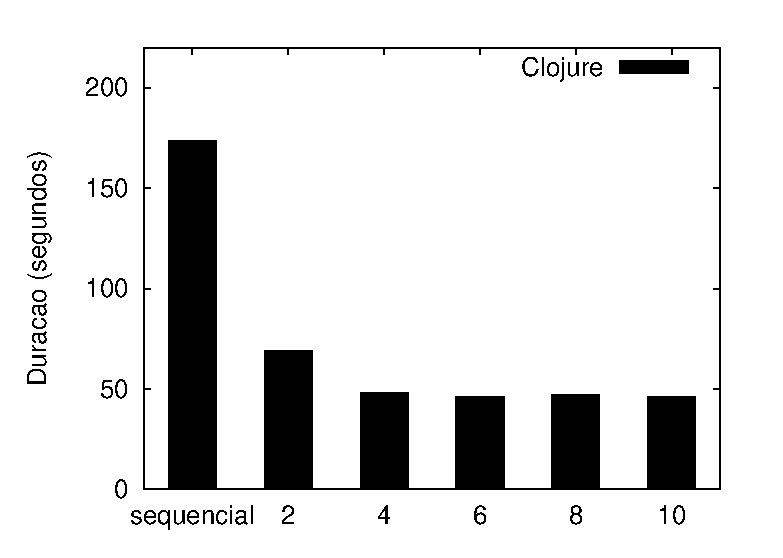
\includegraphics[scale=0.63]{imagens/clojure.eps}
 \end{minipage}
 \caption{Gráficos de comparação entre as versões sequenciais e paralelas}
 \label{fig:clj-hs}
\end{figure}

Depois de realização de alguns \emph{profilings} na versão sequencial em Clojure, foi identificado que o maior gargalo do programa estava acontecendo no processamento dos documentos. O processamento é feito igualmente nas duas versões, os arquivos são lidos em forma de uma única \verb|string|, em seguida são filtrados os caracteres alfanuméricos, depois a capitalização é uniformizada e por último a \verb|string| é quebrada de acordo com os separadores de espaço para gerar uma lista de palavras. O principal problema é que os arquivos em Clojure são lidos como instâncias da classe \verb|String| de Java, porém, quando é feito o processamento dessa \verb|String|, internamente ela é convertida para uma \emph{lazy sequence} \footnote{http://clojure.github.io/clojure/clojure.core-api.html\#clojure.core/lazy-seq}, em seguida, quando a sequência vai ser quebrada ela é transfomada em \verb|String| novamente. Essas transformações degradam bastante o desempenho do programa. Em Haskell esse tipo de problema não acontece pois não há conversões, inclusive, como a leitura de arquivos também acontece de maneira \emph{lazy} em Haskell, mesmo evitando as conversões desnecessárias na implementação em Clojure, o desempenho da versão Haskell no processamento dos documentos provavelmente será melhor.

Embora o provável problema tenha sido identificado e várias alternativas tenham sido tentadas, não foi possível melhorar o desempenho da versão Clojure em tempo hábil para ser incluido no presente trabalho. Entretanto, como pôde ser visto na Figura \ref{fig:clj-hs} a paralelização realizada em ambas as linguagens foram bastante benéficas e diminuiram de maneira considerável o tempo total de execução dos programas, como era esperado.

Ainda com relação à Figura \ref{fig:clj-hs}, é importante notar que a versão Clojure apresentou pouca variação de desempenho a partir de 4 \emph{threads}. Isso pode ser um reflexo do tipo de \emph{thread} que foi utilizada para representar as \emph{threads} de processamento e indexação. Nesse caso, foi utilizado a classe \verb|Thread| de Java que internamente, na máquina virtual de Java, são representadas como \emph{threads} do sistema operacional. Já implementação em Haskell foram utilizadas \emph{threads} criadas por meio da função \verb|forkIO|, que criam \emph{green threads} que são gerenciadas pelo \emph{runtime} da linguagem. As \emph{green threads} são mais leves e sua utilização pode ter impacto direto no aumento do desempenho da aplicação.